\chapter{Introduction}
% -------------------------
%% QUOTE
\vspace*{\fill}
\epigraph{In all matters, before beginning,\\ a diligent preparation should be made.}%
{\textit{De Officiis (44 B.C.), I. 21.}\\ \textsc{Cisero}}
\clearpage{\thispagestyle{empty}\cleardoublepage}
%%
%% Body of the chapter
%%%%%%%%%%%%%%%%%%%%%%
\section{Motivation}
The surge in energy consumption levels is inevitable for modern societies. Their sustainability depends on it. The \usebibentry{EIA2017}{title} report \citeyearpar{EIA2017} published by the \usebibentry{EIA2017}{institution} projects a 28\% increase in world energy consumption between 2015 and 2040, assuming continuous improvement in known technologies based on current trends. As shown in Figure \ref{cht:energySources}, the consumption of ``petroleum and other liquid fuels" alone will grow by 18\%, which will account for 31\% of total world energy consumption in 2040.

\begin{figure}[b!]
    \centering
    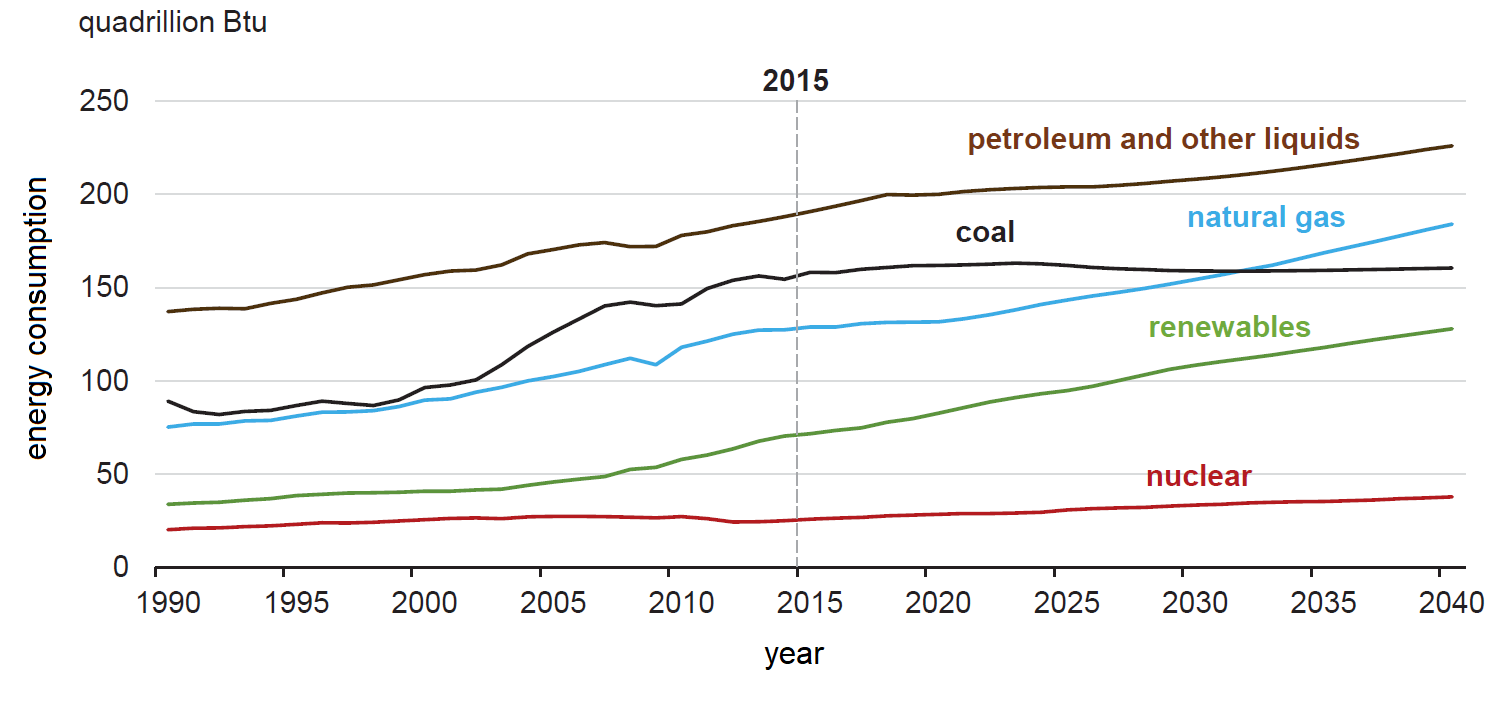
\includegraphics[width=\textwidth]{img/cht/chtEiaEnergy.png}
    \caption{World energy consumption by energy source \citep{EIA2017}}
    \label{cht:energySources}
\end{figure}

It is becoming more and more challenging to meet the ever-increasing demand for petroleum. Most of the existing major oilfields are already at a mature stage and the number of new significant discoveries per year is decreasing. Therefore, at this point in time, it is crucial to focus on methods of improving petroleum production from existing reservoirs. A big subset of such methods fall under the category of Enhanced Oil Recovery (EOR).

Challenges and technology gaps within EOR, \index{EOR!challenges} which need to be addressed in the coming research programs, have been identified in the OG21 strategy document on ``Exploration and Increased Recovery" \citep{OG21}: In particular, there is a need for more cost-efficient EOR chemicals, and to assure environmentally acceptable methods to avoid unwanted discharge to sea. Improved petroleum resource exploitation by EOR has also been given special attention in a report on increased recovery in the Norwegian Continental Shelf by the Norwegian Department of Oil and Energy \citep{Am2010}. There is therefore a clear need for increased competence in new technologies in the field of EOR. 

There has recently been an increasing interest in applying nanotechnology to EOR but still many topics are uncovered. Nanotechnology, \index{Nanotechnology} which has mainly been developed in mechanical engineering, medicine and biological sciences, is expected to have a large potential for EOR applications. This technology has a wide range of applications relevant to EOR, from employing general concepts and principles of nanotechnology, to advanced reservoir monitoring using nano-sensors and nano-analysis, to more specific technologies which make up for the shortcomings in traditional EOR methods \citep{Fletcher2010, Ayatollahi2012, Cocuzza2011}. The latter includes tailoring chemical molecules for more efficient EOR, as well as smart and more effective delivery of EOR agents. Such technologies as efficient drug delivery in the human body may be applied to improve efficiency in chemical flooding.

This PhD work is part of the HyGreGel\index{HyGreGel|(} (Hybrid Green nano-Gels) project. The HyGreGel project addresses the need for more efficient water diversion techniques by improved in-depth placement of gelling chemicals to increase waterflood recovery and reduce unwanted water circulation in heterogeneous reservoirs. The project recognizes the environmental challenges using chemicals and emphasizes the development of green chemical systems for such applications.
\section{Problem formulation}

Incremental recovery from water diversion is generally expected to be merely 2\% above standard water flooding \citep{OG21}. The main objective of HyGreGel is thus 
\begin{tcolorbox}
to improve incremental recovery from water diversion by developing and testing innovative hybrid (polymer + nanoparticle) gels.
\end{tcolorbox}
A thorough study of the effect of surface functionalities of the nanoparticles and their reactivity with the polymers will enable great improvements in controlling gel formation. This can be achieved by learning the scientific reasons behind the experimental results and understanding the kinetics of transport of nano-gels through porous media. Hence,  HyGreGel will contribute to making nanotechnology the next-generation EOR method.

The sub-goals of HyGreGel are:
\begin{enumerate}
    \item To study the effect of functional nanosized particles on the gel formation with polymers by cross-linking, and their transport through the oil reservoir.
    \item To synthetize and further develop  hybrid materials, both in terms of functionality and size.
    \item To investigate the reactivity of the nanosized particles with polymers, ensuring controlled gelling for several weeks and possibly months to assure in-depth placement of gels.
    \item To create basic knowledge on controlled release of encapsulated active components.
    \item To study the effect of real reservoir parameters such as temperature, pressure, brine salinity, and presence of crude oil on gel strength and gel stability and optimize the operational parameters.
    \item To study the integration of hybrid materials in industrial EOR.
\end{enumerate}

The results from HyGreGel will provide an understanding of how the nanoparticles affect the gel properties and their transport mechanism through the oil reservoir. They will also take major steps toward a robust design and manufacturing of hybrid gels. HyGreGel will keep the advantages of polymer materials (flexibility, processability and low cost) and make some improvement in EOR by integrating hybrid nanoparticles in the polymer. \index{HyGreGel|)}

\section{Sub-projects}
The scientific work in the project was done through four sub-projects (SP). The research tasks and scientific methods for each of the SPs are described below.
\subsection{Hybrid materials as sweeping efficiency modifier (SP1)}
SP1 was performed at the Department of Materials and Nanotechnology at SINTEF Industry. The approach was to use FunzioNano\texttrademark (FN)\index{FunzioNano} particles with functional groups having the ability to react with polymers causing cross-binding and gelling. 

Hybrid materials based on FunzioNano are multifunctional nanoparticles which can provide significant benefit in EOR. FunzioNano with blocked functional groups can be used as a latent cross-linker for polymers which are made from renewable resources, e.g. cellulose based polymers. FunzioNano cross-linker and polymer are injected as a formulation at the same time. Hydrolysis within the requested time window leads to de-blocking of the functional groups and thereafter fast and efficient gelation by cross-linking of Funzionano and polymer, e.g. through ionic bond formation between amine functionalities on FunzioNano and carboxylic functionalities on cellulose. The time window for de-blocking FunzioNano can be adjusted by the type and the amount of hydrolysis catalyst. As an additional benefit cross-linked FunzioNano and polymer can provide a more hydrophobic gel than the components themselves. Motion of water could therefore be more efficiently hindered than motion of produced oil which would be suitable for partially blocking gels that can transport the remaining oil. FunzioNano can to a significant extent be manufactured from renewable resources. In case of un-desired spill, FunzioNano is degradable after being highly diluted with water. Computer modelling of the degradability of highly diluted FunzioNano is currently performed in collaboration with Université de Savoie, France [22, 23].


The FN particles are based on nano-sized silica particles with functional groups given specific properties.


\section{Contributions and scope of the PhD work}

As mentioned earlier, this PhD work is a subset of the greater HyGreGel project. Therefore, it is important to clearly identify the scope of this work. The primary contributions are as follows:

\begin{enumerate}
    \item Different types of Functionalized Silica Nanoparticles synthesized by SINTEF Industry in Oslo were tested to identify the ones which create the most stable gels when combined with polymer at elevated temperatures.
    \item Polymer and nanoparticle transport was investigated through core flooding tests with several configurations.
    \item A numerical model developed at SINTEF industry was first tuned to match the results from experiments and thereafter used to simulate transport and gelation of particles in field scale
\end{enumerate}
